\section{Strømforsyning på bil}

Bilens strømforsyning er som førnævnt designet ud fra princippet om en buck converter. Buck converteren fungerer overordnet set ved at en PWM-styret mosfet eller anden form for transistor lukker op og i for en høj spænding ved meget høj frekvens. 
Dette midles herefter i et 2. ordens lavpasfilter.
Den resulterende strøm ledes herefter igennem en diode, så der er en lukket sløjfe i kredsløbet, selvom transistoren er off.

\begin{figure}[h]
\centering
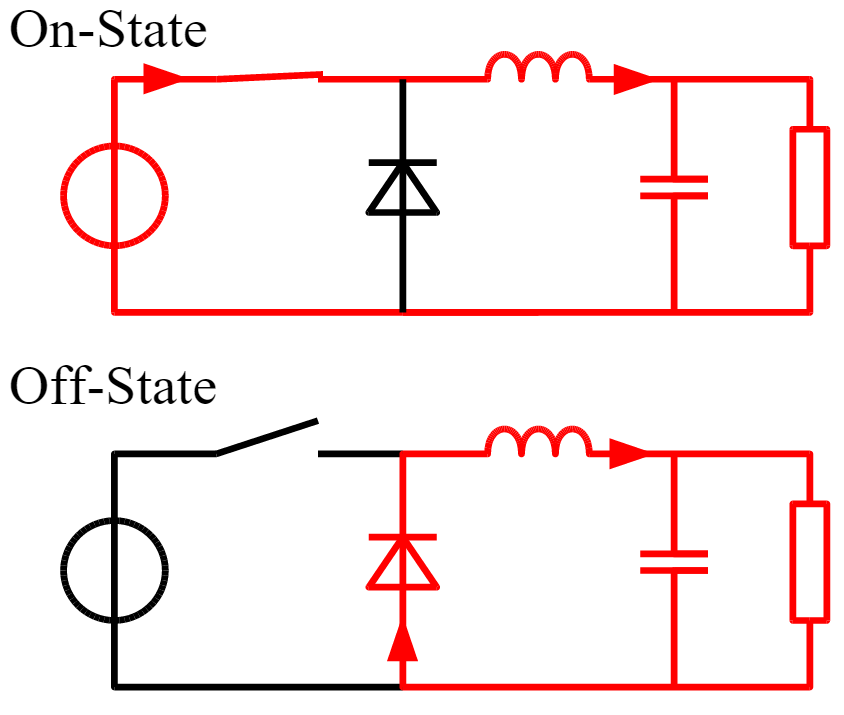
\includegraphics[width=\textwidth * 1/2]{../fig/billeder/buck_circuit_diagram}
\caption{Princippet for en buck converter, figur venligst lånt fra Wikipedia}
\label{fig:buck_conv}
\end{figure}

I figur \ref{fig:buck_conv} vises princippet om en buck converter. 
Det ses hvordan strømmen løber når transistoren er hhv. on og off.
Det mest væsentlige ift. EMC-problematik ligger i de flanker, som opstår når transistoren går on eller off, da disse går fra stel til forsyningsspænding på meget kort tid og ved meget høj skiftefrekvens.
Da dette sker ved 100 kHz i dette system producerer dette ikke blot støj ved 100 kHz, men også ved højere harmoniske frekvenser af de 100 kHz.
\clearpage

\begin{landscape}
\begin{figure}[h]
\centering
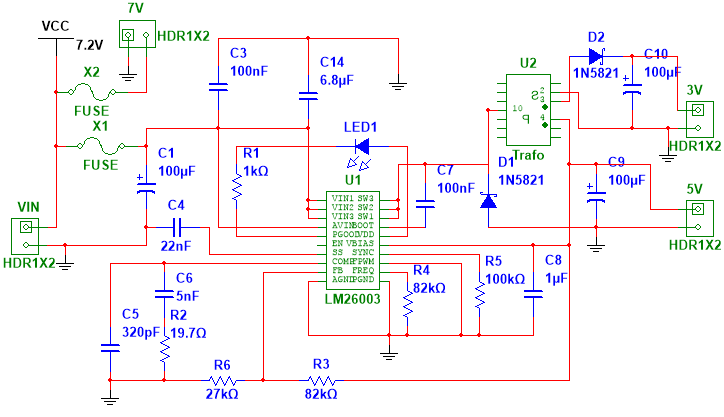
\includegraphics[height=\textwidth -3.2 cm]{../fig/diagrammer/bil/psu_kredsloeb}
\caption{Kredsløbsdiagram for strømforsyning}
\label{fig:psu_kredsloeb}
\end{figure}
\end{landscape}

\clearpage

På figur \ref{fig:psu_kredsloeb} ses hele kredsløbet for bilens strømforsyning. 
Der er en mindre afvigelse i dette design ift. ''standard'' buck converteren i form af en ekstra udgang på 3V.
Dette medfører at der er tre strømloops, hvor der fremkommer højfrekvente signaler.
I figur \ref{fig:psu_kredsloeb_EMC} ses disse indrammet.

Hvis man kikker på den blå strømsløjfe handler det om den vekselstrøm der løber fra batteriet/kondensatoren på indgangen og ud til udgangskondensatoren når transistoren skifter mellem ON og OFF. 
Denne strøm er både højfrekvent og relativt høj i spænding og der er i designet derfor forsøgt at mindske arealet sløjfen dækker over.

Den orange sløjfe viser den skiftende strøm der går gennem dioden og optages af kondensatoren.
Når transistoren er ON løber strømmen gennem IC'en og når transistoren er OFF løber den via dioden.
Måden støjen fra dette reduceres på er ved at mindske arealet for strømloopet.

Til sidst er der den grønne strømløkke, som i denne applikation ikke fører en særlig stor strøm (under 100 mA) og der vurderes ikke at der er de helt store EMC-mæssige problemer fra denne. 
Den er dog værd at tage med, da princippet og frekvenserne er lig de andre to sløjfer.

Udover de markede sløjfer findes der ligeledes fløjfer ved tilbagekobling og stabilisering af udgangssignalet tilbage til IC'en, men disse er af lave strømme og spændinger og er derved ikke betragtet som værende væsentlige i EMC-mæssige øjemed.

\clearpage

\begin{landscape}
\begin{figure}[h]
\centering
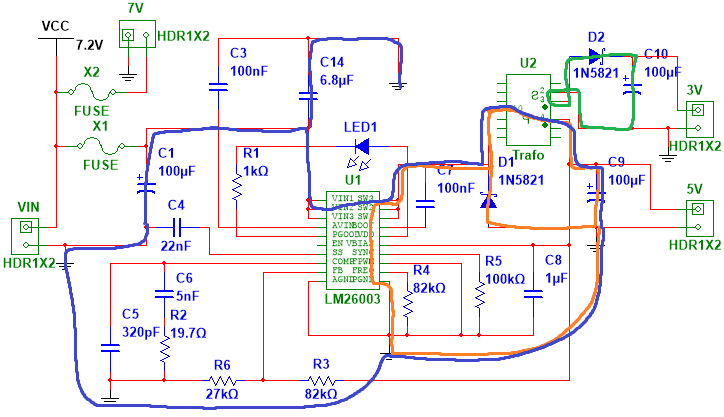
\includegraphics[height=\textwidth -3.2 cm]{../fig/diagrammer/bil/psu_kredsloeb_EMC}
\caption{Kredsløbsdiagram for strømforsyning med strømsløjfer indtegnet}
\label{fig:psu_kredsloeb_EMC}
\end{figure}
\end{landscape}

\clearpage

I figur \ref{fig:psu_pcb} ses det implementerede kredsløb på print.
Det er uheldigvis ikke muligt inden afleveringsdatoen for EMC-rapporten at få printet produceret, så de overvejelser der er gjort i dette afsnit betrates som værende endelige.

Printet er som udgangspunkt lagt ud således at strømsløjferne vedr. output alle er placerede i højre side af printet, tæt sammen med bredde printbaner. 
Returstrømme går via stelplan på bagsiden, hvilket vil sige at arealet på hver strømsløjfe minimeres så vidt som muligt.
Forsyningsstrømmen til IC'en samt direkte udgang er trukket op i øverste venstre side og er derved, på samme vis som udgangssløjfer, langt fra den mere følsomme elektronik i bunden af printet. 
Der er så vidt muligt taget hensyn til at signalbaner og forsyningsbaner (både input og output) ikke er lagt oveni hinanden eller tæt på hinanden. 
Dette minimerer for stelplanets side problemet ved impedans i fælles strømvej. 
Udover dette sker der også en mindre kapacitiv kobling på det vis.

For at mindske højfrekvente strømsløjfer er afkoblingskondensatorer placeret så tæt på de komponenter de skal afkoble som muligt. Dette ses ved C9, C10, C1 og C11-12.

\clearpage

\begin{landscape}
\begin{figure}[h]
\centering
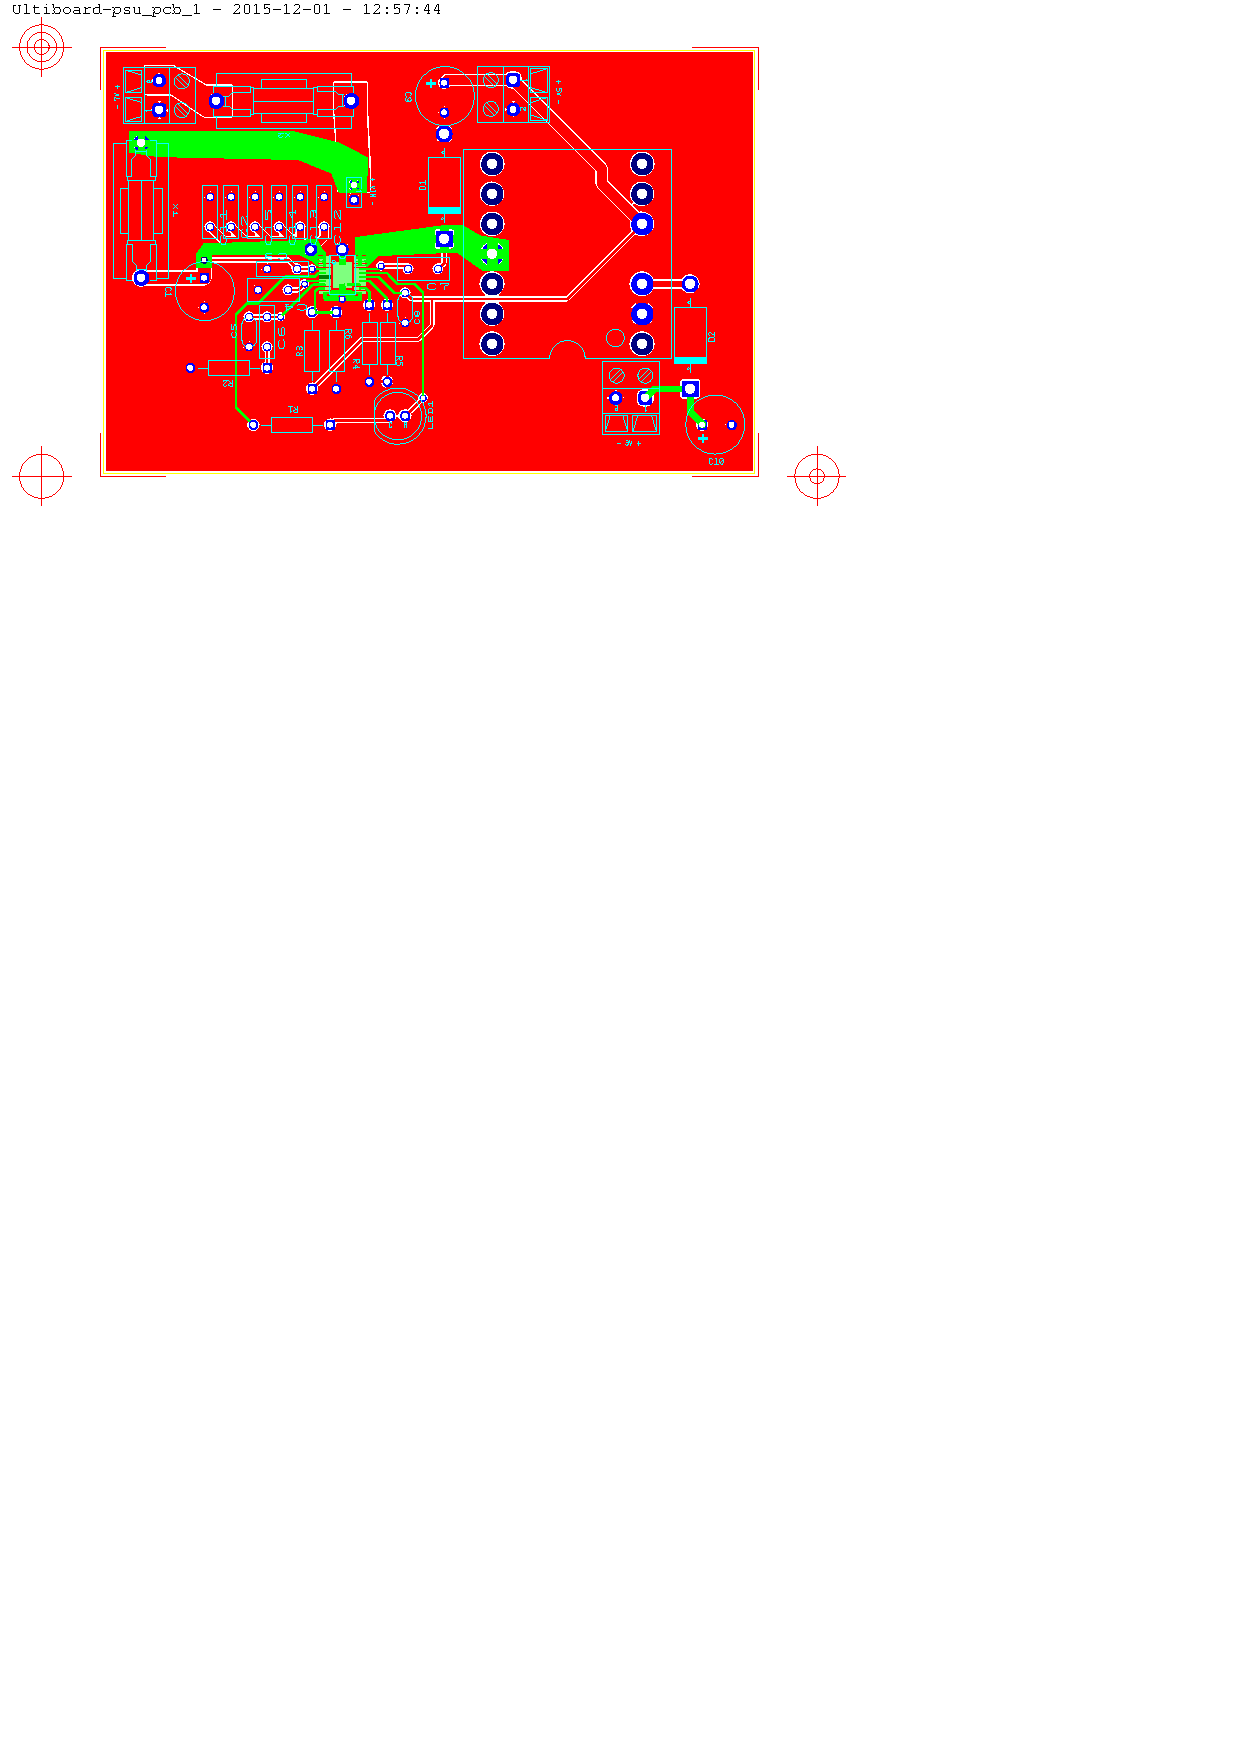
\includegraphics[height=\textwidth-2.5cm, clip=true, trim=50 615 234 25]{../fig/diagrammer/bil/psu_pcb_twoside}
\caption{Kredsløbsdiagram for strømforsyning med strømsløjfer indtegnet}
\label{fig:psu_pcb}
\end{figure}
\end{landscape}


